\section{Linear Regression}

\subsection{Introduction to Linear Regression}

\begin{definition}{Linear Regression}
    Discover the parameters of the straight-line equation that best fits the data points.
    \begin{itemize}
        \item $\bar{x}$ is the mean value of $x$
        \item $\bar{y}$ is the mean value of $y$
    \end{itemize}
    $$
    b=\frac{\sum_{i=1}^n\left(x_i-\bar{x}\right)\left(y_i-\bar{y}\right)}{\sum_{i=1}^n\left(x_i-\bar{x}\right)^2}, \quad a=\bar{y}-b \bar{x}, \quad y=a+b x
    $$
    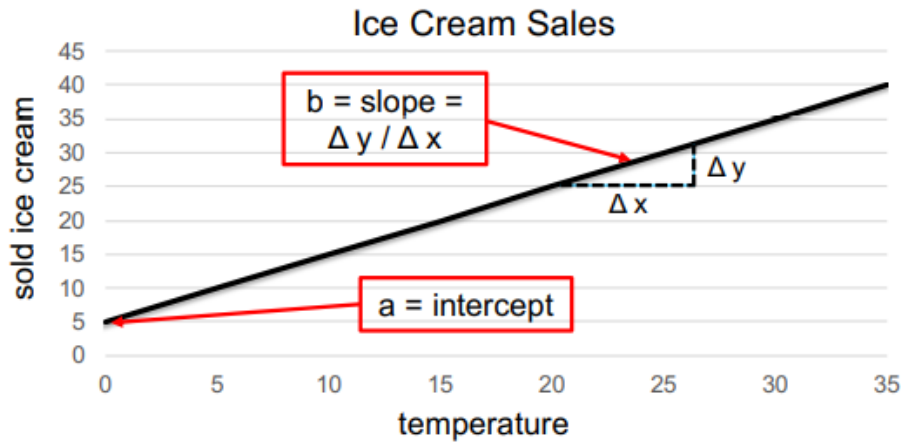
\includegraphics[width=0.8\linewidth]{linear_regression_icecream.png}

    Usage: smooth out noise, fill in missing values, predict future/unknown values
\end{definition}

\begin{formula}{Linear Regression Formula}\\
$$b = \frac{\sum_{i=1}^{n}(x_i - \bar{x})(y_i - \bar{y})}{\sum_{i=1}^{n}(x_i - \bar{x})^2}$$
$$a = \bar{y} - b\bar{x}$$
$$y = a + bx$$
\end{formula}

\subsection{Univariate vs Multivariate Linear Regression}

\begin{concept}{Univariate Linear Regression}\\
In Univariate (Simple) Linear Regression, the output depends on one input variable $x$, and the hypothesis is a linear combination:
\[h_{\theta_0,\theta_1}(x) = \theta_0 + \theta_1 x\]
where $\theta_0$ represents the intercept with the y-axis and $\theta_1$ represents the slope of a straight line.
\end{concept}

\begin{example2}{Univariate Linear Regression Example}\\
    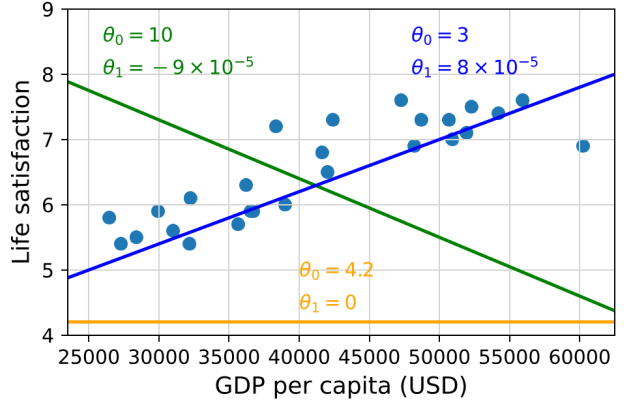
\includegraphics[width=0.6\linewidth]{univariate_linear_regression.png}
\end{example2}

\begin{concept}{Multivariate Linear Regression}\\
Multivariate (Multiple) Linear Regression extends the simple model to handle multiple predictors:
\[\hat{y}^{(m)} = h_\theta(x^{(m)}) = \theta_0 + \theta_1 x^{(m)}_1 + \theta_2 x^{(m)}_2 + \ldots + \theta_N x^{(m)}_N = \theta^T X_{m,:}\]
This can be expressed compactly in matrix form:
\[y = X\theta + \varepsilon\]
where $X$ is the design matrix, $\theta$ is the parameter vector, $y$ is the output vector, and $\varepsilon$ is the error term.
\end{concept}

\begin{example2}{Multivariate Example}\\
Find regression equation $\hat{y} = b_0 \ldots$ to predict test score, based on IQ and the number of study hours.
\begin{itemize}
    \item $b_n =$ Regression coefficients
    \item $x_n =$ Features
    \item $\hat{y} = b_0 + b_1x_1 + b_2x_2$
\end{itemize}
\end{example2}

\subsection{Cost Function and Optimization}

\begin{concept}{Cost Function for Linear Regression}\\
We use the Residual Sum of Squares (RSS) to measure how well our model fits the data:
\[J(\theta_0, \theta_1) = \frac{1}{2M}\sum_{m=1}^{M}(y^{(m)} - \hat{y}^{(m)})^2\]
This is also called the Least Squares Approach.
\end{concept}

\begin{formula}{Normal Equation}\\
For linear regression, we can directly compute the optimal parameters using:
\[\theta = (X^T X)^{-1}X^T y\]
This gives the exact solution without requiring iterative approximation.
\end{formula}

\begin{formula}{Matrix Solution}\\
To find the regression coefficients $b$ we need to solve the following equation:
$$\vec{b} = (X'X)^{-1}X'Y$$
\end{formula}

% NOTE: Add matrix calculation example showing X matrix, Y vector, and solution

\subsection{Training Linear Regression Models}

\begin{KR}{Training a Linear Regression Model}
\paragraph{Steps for training linear regression models}
\begin{enumerate}
    \item Collect your training data consisting of feature vectors $x^{(m)}$ and target values $y^{(m)}$
    \item Decide whether to use the normal equation or gradient descent:
    \begin{itemize}
        \item Normal equation: Use for datasets with fewer than 20,000 features or samples
        \item Gradient descent: Use for larger datasets
    \end{itemize}
    \item For normal equation:
    \begin{itemize}
        \item Construct design matrix $X$ with rows as samples, adding a column of 1s for the intercept term
        \item Calculate $\theta = (X^T X)^{-1}X^T y$
    \end{itemize}
    \item For gradient descent:
    \begin{itemize}
        \item Initialize parameters $\theta$ randomly
        \item Update parameters iteratively using gradient descent until convergence
    \end{itemize}
    \item After training, predict using $\hat{y} = \theta^T x$
\end{enumerate}
\end{KR}

\begin{example2}{Linear Regression Example}
Consider predicting life satisfaction based on GDP:
\begin{itemize}
    \item Input feature: GDP per capita (USD)
    \item Output: Life satisfaction score (1-10)
    \item Training the model gives us parameters $\theta_0 = 3.0$ and $\theta_1 = 8 \times 10^{-5}$
    \item For a country with GDP = 45,000 USD, we predict:
    $\hat{y} = 3.0 + (8 \times 10^{-5}) \times 45000 = 3.0 + 3.6 = 6.6$
\end{itemize}
\end{example2}

\subsection{Mean Square Error (MSE)}

\begin{KR}{MSE Calculation}\\
\paragraph{Step 1}
Find the linear regression line

\paragraph{Step 2}
Insert your $X$ values into the linear regression equation to find new $Y$ values $Y'$

\paragraph{Step 3}
Subtract the new $Y'$ value from the original $Y$ to get the error

\paragraph{Step 4}
Square the errors, add up the errors and calculate the mean
\end{KR}

\begin{example2}{MSE Example}\\
The following regression lines are given:
\begin{itemize}
    \item $y_1 = 9.2 + 0.8x$
    \item $y_2 = 9.1 + 0.75x$
\end{itemize}

Calculate the MSE for the given $X$ and $Y$ values:
$$MSE_1 = 6.08 = \frac{6.67 + 0.36 + 14.44 + 1 + 7.84}{5}$$
$$MSE_2 = 11.61 = \frac{0.12 + 8.41 + 37.8 + 11.56 + 0.12}{5}$$
\end{example2}

% NOTE: Add MSE calculation table showing X, Y, Y1', e1, e1², Y2', e2, e2² columns

\subsection{Evaluating Regression Models}

\mult{2}

\begin{theorem}{Evaluation Metrics for Regression}\\
Common metrics for evaluating regression models include:\\
    Mean Absolute Error: 
    $$MAE = \frac{1}{I} \sum_{i=1}^{I} |y^{(i)}-\hat{y}^{(i)}|$$
    Mean Squared Error: 
    $$MSE = \frac{1}{I}\sum_{i=1}^{I}(y^{(i)}-\hat{y}^{(i)})^2$$
    Root Mean Squared Deviation: 
    $$RMSD = \sqrt{MSE} = \sqrt{\frac{1}{I}\sum_{i=1}^{I}(y^{(i)}-\hat{y}^{(i)})^2}$$
\end{theorem}

\begin{theorem}{Coefficient of Determination}\\
The Coefficient of Determination $R^2$ measures the fraction of the variance explained by the model:
\[R^2 = 1 - \frac{SS_{res}}{SS_{tot}}\]
Residual sum of squares:
$$SS_{res} = \sum_i (y^{(i)} - \hat{y}^{(i)})^2$$
Total sum of squares:
$$SS_{tot} = \sum_i (y^{(i)} - \mu_y)^2$$
$R^2 = 1$ means a perfect fit, while $R^2 = 0$ means the model performs no better than predicting the mean.
\end{theorem}

\multend

\subsection{Assumptions and Residual Analysis}

\begin{concept}{Assumptions in Linear Regression}
\begin{itemize}
    \item \textbf{Linearity}: \\The relationship between X and y is linear
    \item \textbf{Independence}: \\The residuals are independent of each other
    \item \textbf{Normality}: The expected output values are normally distributed
    \item \textbf{Homoscedasticity}: The variance of the residual is the same for any value of X
\end{itemize}
These assumptions can be verified visually using residual plots.
\end{concept}

\begin{corollary}{Residual Analysis}\\
Residual plots help evaluate model quality:
\begin{itemize}
    \item \textbf{Random scatter}: \\Suggests good model fit
    \item \textbf{U-shaped pattern}: \\ Suggests non-linear relationship
    \item \textbf{Funnel shape}: \\ Suggests heteroscedasticity
    \item \textbf{Cyclic pattern}: \\ Suggests seasonality or auto-correlation
\end{itemize}
\vspace{1mm}
Examining residuals can indicate model weaknesses and suggest improvements.
\end{corollary}

\begin{KR}{Interpreting Regression Results}
\paragraph{Examine coefficient values}
\begin{itemize}
    \item Sign indicates direction of relationship (positive or negative)
    \item Magnitude indicates strength of relationship
    \item For standardized features, directly compare coefficient magnitudes
\end{itemize}

\paragraph{Assess model fit}
\begin{itemize}
    \item $R^2$ close to 1 indicates good fit
    \item Low MSE indicates accurate predictions
    \item Check residual plots for patterns
\end{itemize}

\paragraph{Check for violations of assumptions}
\begin{itemize}
    \item Non-linear patterns in residual plot suggest linearity violation
    \item Residuals changing with fitted values suggest heteroscedasticity
    \item QQ-plot deviating from straight line suggests non-normality
\end{itemize}

\paragraph{Consider feature importance}
\begin{itemize}
    \item Features with larger coefficients have greater impact
    \item Statistical significance (p-values) indicates confidence in relationship
\end{itemize}
\end{KR}

\subsection{Logistic Regression}

\begin{definition}{Logistic Regression}\\
Predicts if something is true or false. It provides probabilities $p$ and classifies new samples using continuous and discrete measurements.
\end{definition}

\begin{formula}{Logistic Function}\\
$p = \frac{1}{1 + e^{logit}}$
\end{formula}

\begin{example2}{Logistic Regression Example}\\
$p = \frac{1}{1 + e^{-(b_0+b_1x)}}$

Probability $p$ of passing exam:
$\frac{1}{1 + e^{-(-4.0777+1.5048 \cdot Hours)}}$

\begin{itemize}
    \item Studying 2 hours $\rightarrow$ $p = 0.26$
    \item Studying 4 hours $\rightarrow$ $p = 0.87$
\end{itemize}
\end{example2}

% NOTE: Add comparison diagram showing Linear Regression vs Logistic Regression curves

\begin{example2}{Making Predictions with Linear Regression}\\
Suppose we've trained a multivariate linear regression model to predict house prices based on size (sq ft), number of bedrooms, and age (years). Our trained model has parameters:
\begin{itemize}
    \item $\theta_0 = 50,000$ (intercept)
    \item $\theta_1 = 100$ (coefficient for size)
    \item $\theta_2 = 5,000$ (coefficient for bedrooms)
    \item $\theta_3 = -200$ (coefficient for age)
\end{itemize}
\tcblower
For a house with 1,500 sq ft, 3 bedrooms, and 25 years old, we predict:
\begin{align*}
\hat{y} &= \theta_0 + \theta_1 \times \text{size} + \theta_2 \times \text{bedrooms} + \theta_3 \times \text{age} \\
&= 50,000 + 100 \times 1,500 + 5,000 \times 3 + (-200) \times 25 \\
&= 50,000 + 150,000 + 15,000 - 5,000 \\
&= 210,000
\end{align*}
So, the predicted price is \$210,000.
\end{example2}